\documentclass[../Main.tex]{subfiles}
\begin{document}
\subsection{Model comparison}
We begin experiments by comparing style transfer features and quality of
original and pruned network. We compare models on detailed styles with complex 
structure (Figure \ref{fig:mosaic1}) and minimalistic, low-entropy styles 
(Figure \ref{fig:mosaic2}). 
        \begin{figure}[h!]
        \centering
            \includegraphics[scale=0.2]{mosaic1.png}
            \caption{Comparison of original and pruned network on complex styles. 
            For every pair of rows original model's results are placed in the
            top row and pruned model's results in bottom row.
            }
            \label{fig:mosaic1}
        \end{figure}
As can be seen, pruned model performs on par with the original on complex styles.
The only difference we notice for the first style is slightly lighter hue of sofa
in the dog photo. Otherwise it's hard to find any differences in this column.
In the second column the red jackets in kayak image stand out. This certainly is a drawback,
considering image was supposed to imitate a sketch. Area under a bridge in last 
image is also less detailed and darker. In general small model, as expected,
seems more likely to discard small details - compare surface of water in kayak image
or elephant's back in first image. For styles with one dominating color, smaller
model produces more uniform distribution of colors. It's visible in virtually
all images in the last column; in this case images seem to be "watered down".
Both of these traits are not necessarily drawbacks, for example the blue area
under the bridge in last image of last column looks less coherent than darker version
produced by small model. Discarding details might even be desirable for many styles.

        \begin{figure}[h!]
        \centering
            \includegraphics[scale=0.2]{mosaic2.png}
            \caption{Comparison of original and pruned network on simple styles. 
            For every pair of rows original model's results are placed in the
            top row and pruned model's results in bottom row.
            }
            \label{fig:mosaic2}
        \end{figure} 
 
We now compare networks on very simple styles. In degenerate case of entirely black
style image they perform almost the same. Original model preserves a bit more 
structure, though it might not be visible. It makes sense results are "empty"
since black color is represented by $0$s and the first convolution layer amounts
just to it's bias. Pruned network performs visibly worse in the second case.
Very low contrast of images makes it hard to recognize the original image, while
the original model has no problem approximately reconstructing content. 
The third column is very informative - even though it consists mostly of 2 colors
(unlike a sketch image where various tones of grey are prevalent) both networks
reconstruct content very well. This tells us structure and presence of some kind
of edges in style image is very important for reconstruction - images in the last
column are more blurry, even though color information is richer.
Fourth column shows smaller model  doesn't work very well when structure of style 
image is very sparse. While original model acts as (not very good) edge detector,
pruned network produces seemingly overexposed images.
Overall pruned model performs visibly worse on styles with very simple structure or no
structure at all. 
\subsubsection{Speedup}
In this section we measure speedup provided by pruning and TensorRT. 
We compare speed gains across different devices by taking measurements on three different
NVIDIA GeForce GPUs of varying computational power. In all tests we use RGB images
of resolution 1024x576. 
\begin{table}
\begin{center}
\begin{tabular}{|c|c|c|c|}
\hline
                   & 940M & 960 & 1080 Ti \\
                   \hline
 Original model    &  0.75   & 5   & 23 \\
 \hline
 Pruned model      &  4.2    & 22  & 84 \\
 \hline
 Pruned + TensorRT &  7.1    & 26  &67 \\
 \hline
 \end{tabular}
 \end{center}
 \end{table}

\subsection{Style scaling}
\subsection{Color preservation}
\subsection{Video stability}
\subsection{Style and content encoding} \label{two_encoders}
As mentioned in section \ref{network} the encoder had to be copied due to pruning
constraints. Since two resulting encoders were pruned and fine-tuned separately 
their sets of weights are different. In this section we shortly examine effects
of using wrong combinations of encoder in pruned model. Results for four possible combinations
of encoders are presented if Figure \ref{fig:mosaic_asym}.

        \begin{figure}[h!]
        \centering
            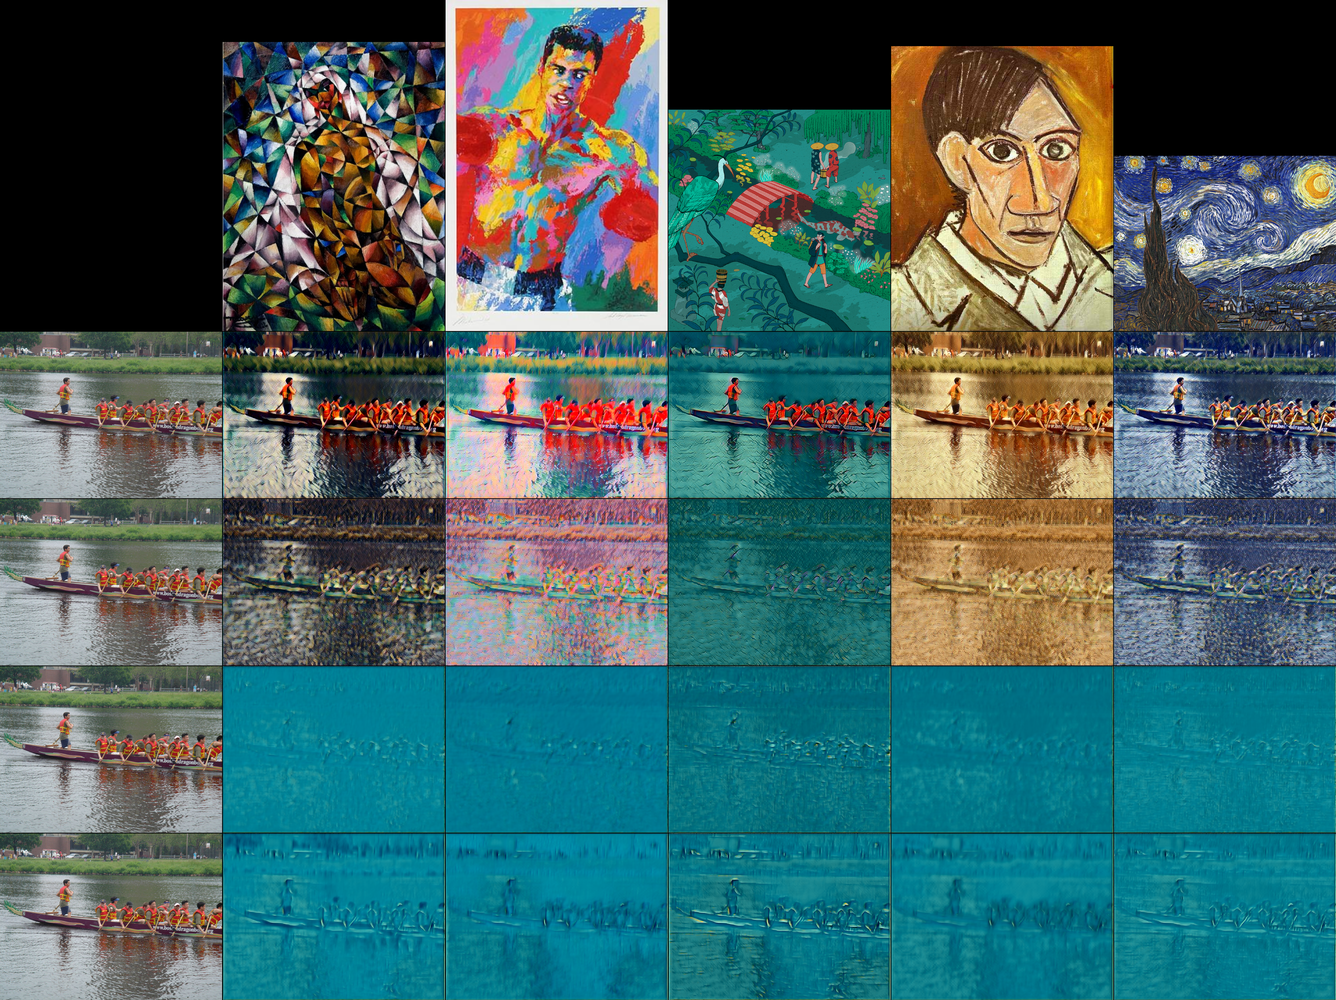
\includegraphics[scale=0.2]{mosaic_asym.png}
            \caption{Comparison of various configurations of network with respect
            to encoder used for encoding style/content image. From top to bottom:
            $S_E(S_I)$ and $C_E(C_I)$, $S_E(S_I)$ and $S_E(C_I)$,
            $C_E(S_I)$ and $S_E(C_I)$, $C_E(S_I)$ and $C_E(C_I)$, where
            $S_E$ and $S_C$ are style and content encoders, $S_I$ and $C_I$ are 
            style and content images.
            }
            \label{fig:mosaic_asym}
        \end{figure}
        
The first row presents default variant with proper configuration. 
We see that while style encoder $S_E$ is able to encode content features to some
degree (2nd row), content encoder $C_E$ fails completely at style extraction
(3rd and 4th row). This is expected, since $C_E$ can usually safely
discard most of color information in content image. On the other hand, $S_E$
should pay attention to both color and shapes. Consequently images in second row
are of a lot worse quality than first row, but content and style are still readily
recognizable. Comparing 3rd and 4th row, we see content 
is reconstructed better in the latter one. Again, this should be the case,
since content is encoded with $S_E$ in 3rd row and with $C_E$ in 4th row.
Since $C_E$ produces more accurate shape encoding than $S_E$, images in 4th row are
sharper and less blurry.
\biblio % Needed for referencing to working when compiling individual subfiles - Do not remove
\end{document}
